\documentclass[12pt,a4paper, openany]{report}
\usepackage[utf8]{inputenc}
\usepackage{amsmath}
\usepackage{amsfonts}
\usepackage{graphicx}
\usepackage[parfill]{parskip}
\graphicspath{ {./images/} }
\usepackage{amssymb}
\usepackage{sectsty}
\author{Alon Engel}
\title{Reversi MinMax- Project Book}
\chapterfont{\centering}



\begin{document}

\maketitle

\tableofcontents

\part{Introduction}

\chapter[Chapter Title]{\centering Project Info}

\section{Game Rules}
\textbf{Reversi} is a two player zero-sum game (meaning one player gains as much as the other player loses as a result of a move). 

\begin{figure}[ht]
\begin{center}
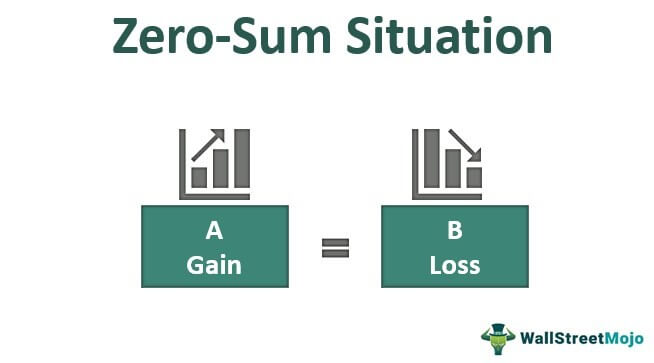
\includegraphics[scale=0.25, width=0.5\textwidth]{Zero-sum-Situation}
\caption{Zero Sum Explanation}
\end{center}
\end{figure}

\pagebreak{}
The board is 8 by 8, and the game pieces are black and white chips, and the starting board is ordered so that there are two pieces (1 black and 1 white, reversed at the 2nd row) at the center of each of the center two rows.

\begin{figure}[ht]
\begin{center}
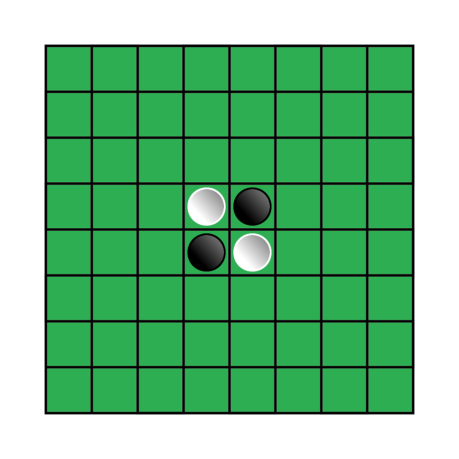
\includegraphics[scale=0.25]{reversi}
\caption{Reversi Starting Board}
\end{center}
\end{figure}

When a chip is placed, all pieces of the opposite color between the placed chip and another chip of the same color are flipped to also become of the same color- This is the main gimmick of the game. A player can only make a move that would result in a flip, if he cannot make one- The turn is surrendered to the other player. If both players cannot make a move- The game is over and the player with the most pieces wins. Pieces can be flipped in a number of direction in one move (see figure 1.4).

\begin{figure}[ht]
\begin{minipage}[c]{0.5\linewidth}
\begin{center}
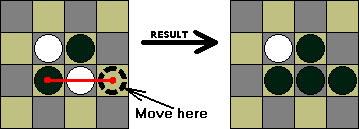
\includegraphics[scale=0.3]{move1}
\caption{Simple Move}
\end{center}
\end{minipage}
\hfill
\begin{minipage}[c]{0.5\linewidth}
\begin{center}
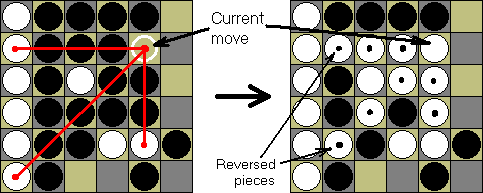
\includegraphics[scale=0.25]{move2}
\caption{More Advanced Move}
\end{center}
\end{minipage}
\hfill
\end{figure}

\pagebreak
\section{The UI}
The UI has two important features to the user. The rest of the features will be discussed more thoroughly later on in the book. The first part is the game board, which looks standard and has indications for what moves can be made and how many pieces can be eaten using that move, and the 2nd one is the indication label which functions both as a winner announcement and to annouce who's turn it is.
\begin{figure}[ht]
\begin{center}
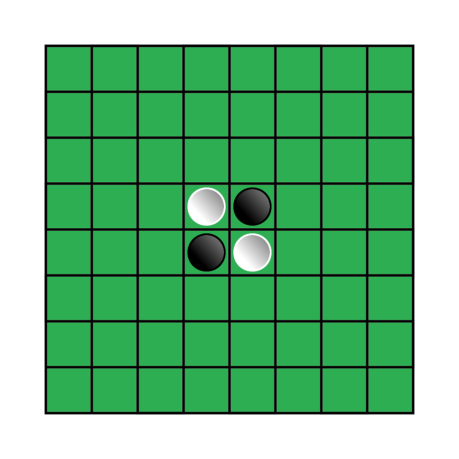
\includegraphics[scale=0.5]{reversi}
\caption{TBA- UI Picture}
\end{center}
\end{figure}

\end{document}}